\documentclass[tikz, border = 5pt]{standalone}

\begin{document}
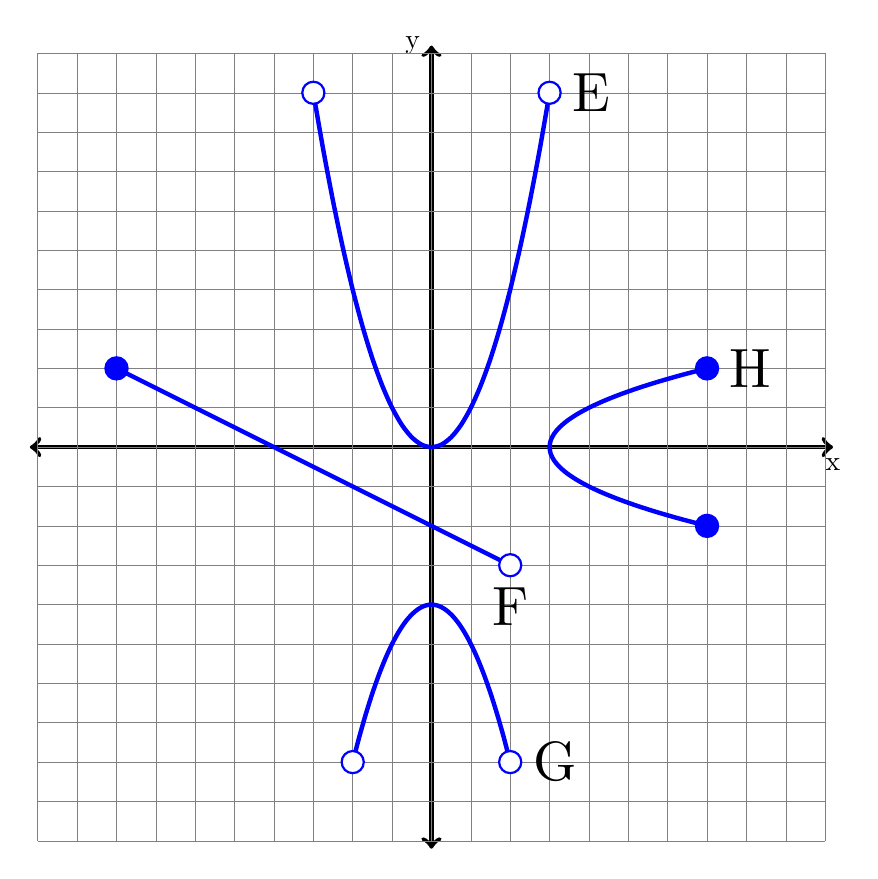
\begin{tikzpicture}
% axis
  \draw[ultra thick, <->] (0, -5.1) -- (0, 5.1) node[left, black, scale=1] {y};
  \draw[ultra thick, <->] (-5.1, 0) -- (5.1, 0) node[below, black, scale=1] {x};

  % grid
  \draw[help lines, step = 0.5cm] (-5, -5) grid (5, 5);

\draw[ultra thick, scale=0.5, domain=-3:3,smooth,variable=\x, blue] plot ({\x},{\x*\x}) node[right, black, scale=2] {E};
\draw [draw=blue, fill=white, thick] (-1.5,4.5) circle (4.0pt);
\draw [draw=blue, fill=white, thick] (1.5,4.5) circle (4.0pt);

\draw[ultra thick, scale=0.5, domain=-8:2,smooth,variable=\x, blue] plot ({\x},{-1/2*\x-2}) node[below, black, scale=2] {F};
\draw [draw=blue, fill=blue, thick] (-4,1) circle (4.0pt);
\draw [draw=blue, fill=white, thick] (1,-1.5) circle (4.0pt);

\draw[ultra thick, scale=0.5, domain=-2:2,smooth,variable=\x, blue] plot ({\x},{-\x*\x-4}) node[right, black, scale=2] {G};
\draw [draw=blue, fill=white, thick] (-1,-4) circle (4.0pt);
\draw [draw=blue, fill=white, thick] (1,-4) circle (4.0pt);

\draw[ultra thick, scale=0.5, domain=-2:2,smooth,variable=\x, blue] plot ({\x*\x+3}, {\x}) node[right, black, scale=2] {H};
\draw [draw=blue, fill=blue, thick] (3.5,1) circle (4.0pt);
\draw [draw=blue, fill=blue, thick] (3.5,-1) circle (4.0pt);

\end{tikzpicture}
\end{document}
